\documentclass[aspectratio=169,11pt]{beamer}

% ============================================================
% SISMID 2026 -- Day 2, 11:00 session
% More novel data streams (S. Yang + C. Djorno)
% Human mobility (ground + air), weather, news alerts.
% Grounded in what the field already uses: GLEAM (Vespignani/MOBS)
% for mobility, Shaman et al. for weather/humidity, HealthMap /
% ProMED / GDELT for news. Hands-on angle: free, scrapable proxies
% for the licensed gold-standard sources.
% Compile: pdflatex more-novel-data-streams.tex  (run twice)
% ============================================================

\IfFileExists{beamerthememetropolis.sty}{
  \usetheme{metropolis}
  \metroset{progressbar=frametitle, sectionpage=progressbar, numbering=fraction}
}{
  \usetheme{Boadilla}
  \usecolortheme{seahorse}
  \setbeamertemplate{navigation symbols}{}
}

\usepackage[utf8]{inputenc}
\usepackage[T1]{fontenc}
\usepackage{tikz}
\usetikzlibrary{arrows.meta, positioning, fit, backgrounds, calc}
\usepackage{xcolor}
\usepackage{listings}

\definecolor{AccentA}{HTML}{2A6F97}
\definecolor{AccentB}{HTML}{C1666B}
\definecolor{AccentC}{HTML}{3B8A5B}
\setbeamercolor{frametitle}{bg=AccentA}
\setbeamercolor{progress bar}{fg=AccentB}

\definecolor{skbg}{rgb}{0.96,0.96,0.94}
\lstdefinestyle{prompt}{
  basicstyle=\ttfamily\scriptsize,
  backgroundcolor=\color{skbg},
  showstringspaces=false, breaklines=true,
  frame=single, framesep=4pt, columns=fullflexible, numbers=none,
}
\lstset{style=prompt}

\tikzset{
  cbox/.style={draw=AccentA, very thick, rounded corners, align=center,
    minimum height=1.0cm, inner sep=6pt, font=\small, fill=AccentA!6},
  sbox/.style={draw=AccentA, thick, rounded corners, align=center,
    minimum height=0.85cm, inner sep=4pt, font=\scriptsize, fill=AccentA!6},
  rbox/.style={draw=AccentB, thick, rounded corners, align=center,
    minimum height=0.85cm, inner sep=4pt, font=\scriptsize, fill=AccentB!8},
  gbox/.style={draw=AccentC, thick, rounded corners, align=center,
    minimum height=0.85cm, inner sep=4pt, font=\scriptsize, fill=AccentC!8},
  flow/.style={-{Stealth[length=3mm]}, very thick, draw=AccentB},
  flowq/.style={-{Stealth[length=2.4mm]}, thick, draw=AccentA!70},
}

\title{More Novel Data Streams}
\subtitle{Mobility, weather, and news, borrowing what the field already uses}
\author{Shihao Yang \quad\textbullet\quad Candice Djorno}
\institute{SISMID 2026 \textbullet\ Day 2, 11:00}
\date{July 21, 2026}

\begin{document}

\begin{frame}
  \titlepage
\end{frame}

\begin{frame}{A different question}
  The streams so far (search, Wikipedia, wastewater) mostly answer \textbf{``how much
  disease is here now?''} These three answer different questions:
  \begin{itemize}
    \item \textbf{Mobility}: where is it \emph{coming from}?
    \item \textbf{Weather}: what is \emph{driving} it?
    \item \textbf{News}: what is \emph{emerging} that has no data yet?
  \end{itemize}
  \vspace{0.3em}
  \begin{block}{Honest framing}
    These are streams other groups pioneered: \textbf{GLEAM} (Vespignani's lab) for
    mobility, \textbf{Shaman et al.} for weather, \textbf{HealthMap / ProMED} for news. We
    credit them, and we show how to reach \emph{free, scrapable} versions with an agent.
  \end{block}
\end{frame}

\begin{frame}{Roadmap}
  \tableofcontents
\end{frame}

% ===============================================================
\section{Human mobility}

\begin{frame}{Disease travels with people, not with distance}
  Epidemics spread along how people actually move. Big, well-connected places seed smaller
  ones (the gravity / metapopulation intuition behind flu spread).
  \begin{itemize}
    \item \textbf{Ground} movement (commuting) drives local, radial spread between nearby
          counties.
    \item \textbf{Air} travel drives long-range importation, seeding distant places.
  \end{itemize}
  \vspace{0.3em}
  \begin{center}
    \itshape So two questions: which neighbors will seed me next, and which far-off places
    import risk to me?
  \end{center}
\end{frame}

\begin{frame}{The gold standard: GLEAM (Vespignani / MOBS lab)}
  The most established mobility-driven epidemic model, and worth knowing by name.
  \begin{itemize}
    \item \textbf{Air travel:} the \textbf{OAG} and \textbf{IATA} databases, roughly 3,800
          airports and 4M+ connections.
    \item \textbf{Ground:} a \textbf{commuting} database from 40+ national statistics
          offices, 78,000+ regions, 5M+ connections, mapped with Voronoi cells around
          airports.
    \item \textbf{Population:} WorldPop / Gridded Population of the World.
  \end{itemize}
  \vspace{0.3em}
  \begin{alertblock}{The catch for a hands-on class}
    OAG, IATA, and SafeGraph are \textbf{licensed}. We cannot scrape them live. So we use
    \textbf{free proxies} and keep cached snapshots of the licensed ones.
  \end{alertblock}
\end{frame}

\begin{frame}[fragile]{Ground mobility you can actually scrape}
  \begin{itemize}
    \item \textbf{US Census LODES} (origin-destination commuting) is free and detailed: who
          lives where and works where, down to the census tract.
    \item \textbf{Google COVID-19 Community Mobility} (archived 2020--2022) and the \textbf{ODT
          Flow Explorer} are free downloads; \textbf{SafeGraph} is licensed, so cached.
  \end{itemize}
  \begin{block}{Prompt}
  \begin{lstlisting}
Using US Census LODES origin-destination data, for Fulton
County, GA, rank the counties that send the most commuters
in. Return the top 10 as a tidy table. These are the
neighbors whose outbreaks tend to reach us first.
  \end{lstlisting}
  \end{block}
\end{frame}

\begin{frame}[fragile]{Air mobility you can actually scrape}
  \begin{itemize}
    \item \textbf{OpenSky Network} exposes real flight data (ADS-B) through a free API, a
          workable stand-in for OAG/IATA to rank inbound connections.
    \item Cross-check which countries a place \textbf{exchanges} with using Wikipedia (a
          trick from our own planning), then reason about importation risk.
  \end{itemize}
  \begin{block}{Prompt}
  \begin{lstlisting}
Using the OpenSky Network API, list arrivals into Atlanta
(ATL) over the past month and tally them by origin
airport and country. Rank the countries that connect to
ATL the most, as a proxy for air-importation risk.
  \end{lstlisting}
  \end{block}
\end{frame}

% ===============================================================
\section{Weather}

\begin{frame}{Weather as a modulator, not a case count}
  Weather does not count cases; it \textbf{shifts the conditions} for transmission.
  \begin{itemize}
    \item \textbf{Influenza:} \textbf{absolute humidity} is the dominant driver. Shaman et
          al. showed virus survival and transmission fall as absolute humidity rises, and
          built humidity-driven flu forecasts.
    \item \textbf{Vector-borne (dengue, Zika):} \textbf{temperature and rainfall} govern the
          mosquito life cycle, so they modulate outbreak timing and size.
  \end{itemize}
  \vspace{0.3em}
  \begin{center}
    \itshape Mauricio picks up the modeling of weather-as-modulator this afternoon; here we
    just get the data.
  \end{center}
\end{frame}

\begin{frame}[fragile]{Weather you can actually scrape}
  \begin{itemize}
    \item \textbf{Open-Meteo} gives free historical and forecast weather with \textbf{no
          key}: ideal for an agent.
    \item \textbf{ERA5} (Copernicus) is the research-grade reanalysis (temperature and dew
          point at 0.25 degrees) behind most humidity studies.
  \end{itemize}
  \begin{block}{Prompt}
  \begin{lstlisting}
Using the Open-Meteo historical API (no key), pull daily
temperature and dew point for Atlanta since 2016. Compute
weekly absolute humidity from them, and overlay it on flu
ED visits so I can see whether low humidity precedes flu
season.
  \end{lstlisting}
  \end{block}
\end{frame}

% ===============================================================
\section{News alerts}

\begin{frame}{News: catching what has no data yet}
  For a genuinely \textbf{emerging} outbreak, there is no search history and no wastewater
  site. The earliest signal is a report.
  \begin{itemize}
    \item \textbf{ProMED} (human-curated, since 1994) and \textbf{HealthMap} (news wires,
          RSS, ProMED, WHO, auto-parsed and geocoded) are the established event-based
          systems. ProMED flagged COVID roughly a day before official notification.
    \item These feed WHO's EIOS and are used by CDC and WHO.
  \end{itemize}
  \vspace{0.3em}
  \begin{center}
    \itshape This is also a stream in Mauricio and Kogan's multi-source COVID forecasting:
    searches + news alerts + GLEAM.
  \end{center}
\end{frame}

\begin{frame}[fragile]{News you can actually scrape}
  \textbf{GDELT} monitors world news in 100+ languages, is 100\% free, and has an API,
  which makes it perfect for an agent. Or point the agent at a news filter directly.
  \begin{block}{Prompt}
  \begin{lstlisting}
Using the GDELT DOC 2.0 API, find news articles from the
past month that mention dengue outbreaks. Return date,
country, and headline; then summarize which countries are
newly reporting activity, as an emerging-outbreak watch.
  \end{lstlisting}
  \end{block}
  \begin{center}
    \itshape Noisy by nature: news reflects attention and reporting, so a human read is part
    of the loop.
  \end{center}
\end{frame}

% ===============================================================
\section{Pulling it together}

\begin{frame}{The pattern behind all three}
  \begin{center}
  \resizebox{0.9\textwidth}{!}{%
  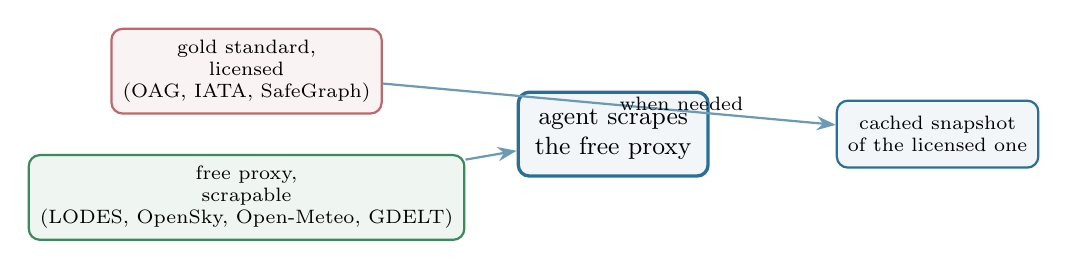
\begin{tikzpicture}[node distance=0.5cm and 1.2cm]
    \node[rbox] (lic) {gold standard,\\licensed\\(OAG, IATA, SafeGraph)};
    \node[gbox, below=of lic] (free) {free proxy,\\scrapable\\(LODES, OpenSky, Open-Meteo, GDELT)};
    \node[cbox, right=1.7cm of lic, yshift=-0.8cm] (a) {agent scrapes\\the free proxy};
    \node[sbox, right=1.6cm of a] (c) {cached snapshot\\of the licensed one};
    \draw[flowq] (free) -- (a);
    \draw[flowq] (lic) -- node[right,font=\scriptsize]{when needed} (c);
  \end{tikzpicture}}
  \end{center}
  \vspace{0.3em}
  \begin{itemize}
    \item Same five-step loop, same verify habit as every other stream.
    \item These are \textbf{context} signals (spread, drivers, emergence), noisier than a
          local case proxy. Treat them as complements, and validate.
  \end{itemize}
\end{frame}

\begin{frame}{Where this connects}
  \begin{itemize}
    \item \textbf{This afternoon:} the network / ARGONet idea borrows signal from neighbors,
          which is exactly what \textbf{ground mobility} tells you to do. Mauricio also covers
          \textbf{weather} and \textbf{news} for emerging outbreaks.
    \item \textbf{Day 3 capstone:} pick the streams that fit your question. Importation risk?
          Use air mobility. Seasonality? Weather. Emerging threat? News.
  \end{itemize}
  \vfill
  \begin{center}
    \itshape You now know the field's established streams by name, and a free, agent-scrapable
    way into each.
  \end{center}
\end{frame}

\begin{frame}{Credits and sources}
  \footnotesize
  \begin{itemize}
    \item \textbf{Mobility / GLEAM:} Balcan et al., \emph{Multiscale mobility networks and
          the spatial spreading of infectious diseases}, PNAS 2009; the GLEAM Project (MOBS
          lab, Northeastern; Vespignani). Data: OAG, IATA, national commuting statistics,
          WorldPop.
    \item \textbf{Free mobility proxies:} US Census LODES; OpenSky Network; Google COVID-19
          Community Mobility Reports (archived); ODT Flow Explorer.
    \item \textbf{Weather:} Shaman \& Kohn (PNAS 2009) and Shaman et al. (PLoS Biology 2010;
          PNAS 2012) on absolute humidity and influenza. Data: Open-Meteo; ERA5 (Copernicus).
    \item \textbf{News:} ProMED (ISID); HealthMap (Brownstein / Freifeld); WHO EIOS; GDELT.
          Multi-source forecasting: Kogan, Santillana et al., \emph{Science Advances} 2021.
  \end{itemize}
\end{frame}

\begin{frame}[standout]
  Questions?\\[0.4em]
  \small Repo: \texttt{github.com/Shihao-Yang/sismid2026}
\end{frame}

\end{document}
